\section{敏感性与可行性检验}

问题一对返航安全余量的离散扫描见图~\ref{fig:sens}。10\%和20\%余量下均需18架次、59.1313~kWh；30\%时组批跳变至20架次、67.2276~kWh；40\%时在“单点直送、货箱不可拆”模型内，S004的14~kg整箱水已没有可行机型，增加架次数也无法恢复该单箱可行性。

\begin{figure}[H]\centering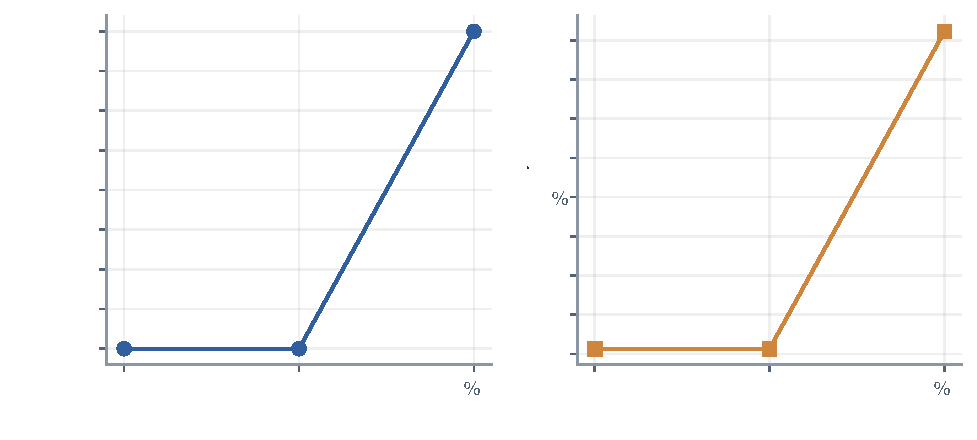
\includegraphics[width=.88\textwidth]{../figures/audit_verified_20260925/q1_sensitivity.pdf}\caption{返航安全余量对单点组批架次和能耗的影响}\label{fig:sens}\end{figure}

在本文明示的水平等效航程加爬升能耗解释下，保持已选路线和时刻不变，将全部水平能耗同乘倍率，逐架次求触及20\%返航储备的临界增幅。表~\ref{tab:energy_stress}显示最紧架次。问题二、三均由A型T010控制，其标称电量余量仅0.01829~kWh，水平耗电增加0.5441\%就会触及储备线；统一上调1\%会使一架次越界。这是固定方案压力检验，不等同于扰动后的重新优化。

\begin{table}[H]\centering\caption{固定航次的能耗扰动临界值}\label{tab:energy_stress}
\begin{tabular}{lrrr}\toprule
方案 & 最紧架次 & 水平项临界增幅 & 同比总能耗临界增幅\\\midrule
问题一 & Q1-07 & 4.1343\% & 4.0155\%\\
问题二 & T010 & 0.5441\% & 0.5107\%\\
问题三 & T010 & 0.5441\% & 0.5107\%\\\bottomrule
\end{tabular}\end{table}

逐箱时限由交接完成时刻独立复算：问题二最紧硬截止提前221.03~s，问题三提前84.65~s；两份主方案的31箱适用硬截止全部满足，64箱非医疗物资亦无迟到、错站或重复交付。最低运输返航SOC均为20.4065\%，问题三最低中继SOC为38.6085\%；实体机、电池和中继组件的占用均不重叠。问题三的4061个连续通信区间全部有链路证书，但最小证明裕量仅0.09378~dB；若额外链路损耗上调0.1~dB，现有证书至少有一段不再成立。这不证明其他站点或时刻无解，只说明本方案必须在现场重新测量和认证。

能源与低碳方面，问题三主方案任务耗电78.8732~kWh，单位货物耗电为0.10405~kWh/kg；节能对照为78.7956~kWh，相差仅0.0776~kWh，代价是全部设备返航晚55.88~s。耗电、单位货物耗电和每kWh完成的配送质量只是任务能源代理指标。附件没有充电效率、电网排放因子和设备全生命周期数据，不能把节电换算为CO$_2$减排。静态DEM、风雨、设备衰减和定位误差亦限制现场外推。

\begin{table}[H]\centering\small
\caption{已完成的参数扰动及固定方案敏感性结论}\label{tab:sensitivity_summary}
\begin{tabular}{lll}\toprule
扰动对象 & 检验范围或阈值 & 已验证影响\\\midrule
Q1返航安全余量 & 10\%--40\% & 30\%增至20架次；40\%出现不可直送整箱\\
Q2水平能耗 & 统一增加0.5441\% & 最紧架次触及20\%返航储备\\
Q3水平能耗 & 统一增加0.5441\% & 最紧架次触及20\%返航储备\\
Q3额外链路损耗 & 增加0.1~dB & 现有连续通信证书至少一段失效\\\bottomrule
\end{tabular}\end{table}
